%
% File:     chapter-scheduler-evaluation.tex
% Author:   awl8049
% Revision: $Revision: 2.1 $
\chapter{Thermal Aware Scheduler Evaluation}
\label{chp:scheduler-evaluation}
We have evaluated our TAS (Thermal Aware Scheduler) using the FreeBSD
operating system run on a commodity server.  Our TAS implementation
modified the existing push migration in FreeBSD's ULE
scheduler~\cite{Roberson2003,McKusick2004,McKusick2004b} to take into
account both thermal behavior and system performance, as elaborated in
Chapter~\ref{chp:schedule}.  PeC data were collected at the user level
through standard tools provided for the data collection purpose by
FreeBSD (i.e., the \texttt{coretemp} and \texttt{hwpmc} kernel
extensions).  They were collected and collated by a FreeBSD kernel
extension, made available to the operating system scheduler for query
when making scheduling decisions (\figurename~\ref{fig:teaplant})

The processor thermal model was calibrated by measuring behavior
outcomes of the testbed with TAS at idle and under high load stress
using common utilities from the FreeBSD regression test suites and
software collections.  The CPU-related behavior of our scheduler was
then characterized using integer and floating point benchmarks from the
SPEC CPU2006~\cite{Henning2006} benchmark suite.  Benchmarks from the
Princeton Application Repository for Shared-Memory Computers (PARSEC)
suite~\cite{Bienia2008} were then evaluated on the testbed to assess TAS
in terms of key metrics of interest (i.e., die temperature and benchmark
run time) under high parallelism in the thread level.

\begin{table}[tbhp] 
\centering
  \caption{Processor used in evaluation}
  \label{tab:hardware}
  \begin{tabular}{l l} 
\hline 
\hline
&\textbf{Dell Precision 490}\\ 
\hline 
CPU&Intel Xeon 5300 (Woodcrest)\\ 
CPU L2 cache&4MB\\ 
Memory&8GB, DDR2 667Mhz with ECC\\
Internal disk&500GB\\ 
Network&1x1000Mbps\\ 
Video&NVIDA Quadro FX3400\\ 
\hline
  \end{tabular}
\end{table}
\section{Experiment Setup}
\label{sec:experiment-setup} 
Experimental evaluation was conducted on our testbed running TAS, with
its hardware specified in Table~\ref{tab:hardware}.  The key metrics of
interest were gathered during the course of application execution.
Power consumed was measured by a WattsUP power meter
\cite{WattsUp2006a}, connected between the AC Main and the server
testbed.  The power meter measured the total and average wattage,
voltage, and amperage over the run of a workload.  The internal memory
of the power meter was cleared at the start of each run and the measures
collected during the runs were downloaded (after execution completion)
from the meter's internal memory into a spreadsheet.

\section{SPEC Benchmark Results and Discussion}
\label{sec:microarch} 
Benchmarks from the SPEC CPU2006 suite \cite{Henning2006} were used to
evaluate the thermal behavior of CPU-bound workloads executed on our
testbed with the TAS scheduler.  The benchmarks were selected to
represent real life applications under various levels of thermal
stress. It has been shown previously \cite{Choi2007,Cher2011} that
significant core-to-core and functional unit-to-functional unit thermal
variations occur on modern processors, with the result that different
workload characteristics have strong influence on the power and thermal
behavior of the processor~\cite{Jimenez2010}.  We thus consider mixing
integer and floating-point SPEC CPU2006 benchmarks for concurrent
execution on the four cores of our testbed processor.  

\begin{table}[t]
  \centering
  \caption{Branch and Memory Access Patters of Evaluation Benchmarks}
  \label{tab:mixstats}
\begin{tabular}{lrrrrr}
\hline
\multicolumn{1}{l}{\textbf{Benchmark}}& \multicolumn{1}{c}{\textbf{Inst Count}} & \multicolumn{1}{c}{\textbf{Branches}}&\multicolumn{1}{c}{\textbf{Loads}} & \multicolumn{1}{c}{\textbf{Stores}} \\
 & \multicolumn{1}{c}{\textbf{(Billions)}}&  &  &  \\
\hline
namd & 2.483 & 4.28\% & 35.45\% & 8.83\% \\
hmmer & 3,363 & 7.08\% & 47.36\% & 17.68\% \\
mcf & 327 & 21.17\% & 37.99\% & 10.55\% \\
milc & 937 & 1.51\% & 40.15\% & 12.98\% \\
\hline
\end{tabular}
\end{table}
Three workload mixes are considered, and they span a range of cases,
including high-IPC/low-IPC, hot/cold thermal profiles \cite{Kursun2008},
and integer/floating-point combinations~\cite{Phansalkar2007} for better
evaluating our scheduler under diverse workload variations.  As
illustrated in Table~\ref{tab:mixstats}, the mix of instructions in the
selected benchmarks benchmark exercises the key components of the
processor, memory, and cache to create workloads with varying levels of
thermal stress. The three workload mixes are as follows: Workload Mix
$A$ = \{\texttt{namd}, \texttt{namd}, \texttt{hmmer}, \texttt{mcf}\},
Workload Mix $B$ = \{\texttt{milc}, \texttt{milc}, \texttt{namd},
\texttt{hmmer}\} and Workload Mix $C$ = \{\texttt{milc}, \texttt{mcf},
\texttt{mcf}, \texttt{hmmer}\}.  For example, Workload Mix $B$ involved
three copies of floating-point benchmarks (i.e., \texttt{milc},
\texttt{milc}, and \texttt{namd}) and one integer benchmark,
\texttt{hmmer}.  The memory intensive benchmarks (for instance, the
\texttt{milc} benchmark) tend to consume more power when executed as
opposed to other benchmarks in the suite while benchmarks with higher
IPC (the \texttt{mcf} and \texttt{hmmer} benchmarks) tends to increase
core on-die temperatures.

\begin{table}[tbp] 
\centering
\caption{Temperature and runtime results under benchmark mixes}
\label{tab:mixwkload}
\begin{tabular}{cllllll} 
\hline
\hline
\textbf{Workload} & \multicolumn{4}{c}{\textbf{Core die temperature reduction}} & \textbf{Runtime}\\
 \textbf{Mix} & \textbf{Core 0} & \textbf{Core 1} & \textbf{Core 2}  & \textbf{Core 3} & \textbf{increase} \\
\hline
$A$ & 2.8$^{\circ}$C & 1.0$^{\circ}$C & 1.7$^{\circ}$C & 2.0$^{\circ}$C & 2.1\% \\
$B$ & 1.0$^{\circ}$C & 0.8$^{\circ}$C & 2.0$^{\circ}$C & 1.1$^{\circ}$C & 2.9\% \\
$C$ & 3.1$^{\circ}$C & 3.3$^{\circ}$C & 3.0$^{\circ}$C & 2.9$^{\circ}$C & 2.5\% \\
\hline
\end{tabular}
\end{table}

It was observed that as execution progressed, the threads of those
benchmarks again tended to pin themselves to particular cores, depending
upon cache and memory utilization of other concurrent threads.  Core
temperatures are reduced under TAS in comparison to those under ULE,
with the reduction amounts listed in Table~\ref{tab:mixwkload} for the
three workload mixes.  Under Workload Mix $C$, for example, TAS lowers
core temperatures by at least 2.9$^{\circ}$C and by as much as
3.3$^{\circ}$C.  The benchmark run times (which reflect performance
degradation) increase negligibly always, ranging from 2.1\% to 2.9\%.

Involving both thermal-aware scheduling and load balancing, TAS compares
favorably with earlier workload migration-oriented methods, with
comparable reductions in average core die temperatures and performance
impact for similar workloads and processors.  Specifically,
Variation-Aware Core Hopping~\cite{Kursun2009} examined both thread
migration, by using off-line profiling of processor thermal variation to
guide assignment of threads to cores, and thread selection, by using the
profiling information to guide scheduling decisions in an enhanced Linux
scheduler.  This technique was demonstrated to lower core temperatures
ranging from 2.0$^{\circ}$C to 5.5$^{\circ}$C with pairs of SPEC CPU2006
benchmarks executed an IBM POWER5 processor with minimal overhead in the
decision process. However, their implementation did not performance
impact of logical cores sharing resources and the related
migration costs entailed by not considering cache affinity in scheduling
decisions.  Meanwhile, Predict-and-Act~\cite{Ayoub2011}
employs a hybrid reactive/proactive migration policy that controls
system fan speeds while scheduling threads at the core level.  This
hybrid method  was shown
to reduce on-die core temperatures by 3$^{\circ}$C to 4$^{\circ}$C on a
"simulated" pair of quad-core Intel Xeon processors (rather than a real
implementation) when executing mixes of SPEC2006 benchmarks similar to
those in our study.

\begin{table}[tbp] 
\centering
 \caption{PARSEC benchmarks used in evaluation}
\label{tab:parsecbench}
\begin{tabular}[bthp]{l l p{5cm}} 
\hline 
\hline 
bodytrack &  & Computer vision image tracking application \\
canneal &  & Simulated annealing chip routing cost computation \\
facesim &  & Physical simulation of facial behavior \\
ferret &  & Content-based similarity search \\
freqmine &  & Simulate FP-growth method for Frequent Itemset Mining \\
streamcluster &  & Online clustering algorithm for data mining \\
swaptions &  & Simulated pricing of portfolio options \\
\hline
\end{tabular}
\end{table}
\section{PARSEC Benchmark Results and Discussion}
\label{sec:mult-behav} 
Selected benchmarks from the PARSEC~\cite{Bienia2008} suite, described
in Table~\ref{tab:parsecbench}, were used to evaluate our TAS as well.
They were compiled with the POSIX \texttt{pthreads} library and executed
using the PARSEC \texttt{native} input sets.  Being parallel workloads
selected from the fields of computer vision, computational finance,
enterprise servers, and animation physics (see Table~\ref{tab:parsecbench}), PARSEC
benchmarks better represent real life applications than SPEC CPU2006 and
can benefit markedly from scheduling their abundant independent threads
freely based on thermal prediction.

\begin{figure}[tbp] 
\centering
  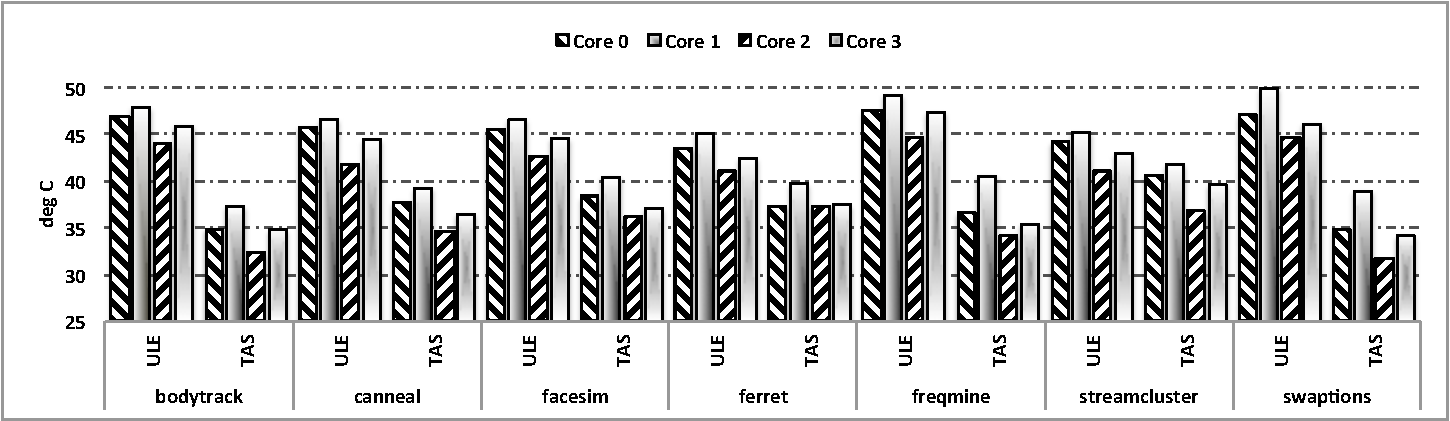
\includegraphics[width=1.0\linewidth,height=2.5in]{parsectemp}
  \caption{Comparison of PARSEC benchmark average core die temperatures
under ULE and TAS schedulers.}
  \label{fig:pbenchmarkt}
\end{figure}
Three behavior metrics of interest under TAS are gathered: (1) the
average core on-die temperature, (2) the benchmark run time, and (3)
mean system power dissipation.  The outcomes of average core on-die
temperatures upon executing those seven PARSEC benchmarks are depicted
in \figurename~\ref{fig:pbenchmarkt}.  As can be seen from the figure,
the core on-die temperatures range from 32$^\circ$C (for Benchmark
\texttt{swaption}) to 42$^\circ$C (for Benchmark \texttt{streamcluster})
under TAS, with \texttt{swaption} and \texttt{bodytrack} (or
\texttt{streamcluster}) experiencing the lowest (or highest) mean
temperature across the four cores.  Temperature outcomes for the same
benchmarks under the classical ULE scheduler are also included in
\figurename~\ref{fig:pbenchmarkt} for comparison.  It is found that
temperature reduction amounts are larger for benchmarks with smaller
working sets (like \texttt{bodytrack} and \texttt{swaptions}).  This is
because such a benchmark has a lower cache requirement \cite{Bienia2011}
and thereby lets TAS schedule threads more freely according to thermal
prediction with negligible performance degradation, resulting in better
temperature reduction.  Consequently, TAS enjoys temperature reduction
by more than 12.8$^{\circ}$C (from 44.8$^{\circ}$C down to
32.2$^{\circ}$C) for the \texttt{swaptions} benchmark.
  
Benchmarks with streaming functions, such as \texttt{facesim},
\texttt{freqmine}, and \texttt{streamcluster}, all have large working
sets, which hinder TAS from scheduling threads freely based on thermal
prediction, since doing so degrades performance considerably.  Hence,
those benchmarks tend to yield less temperature reduction under TAS,
with the average core on-die temperature lowered by 3-6$^{\circ}$C.  

Execution performance (measured in terms of the benchmark runtime) under TAS 
is depicted in \figurename~\ref{fig:pbenchmarkp}.
When compared with the runtime results under ULE included in the figure,
it can be observed that TAS leads to negligible performance degradation,
by no more than 3.3\% for all benchmarks examined except \texttt{streamcluster}.
Considerable performance degradation is seen for Benchmark \texttt{streamcluster},
however, likely due to its high computational intensity as the data set
grows with rising dimensionality and thereby calling for
more synchronization required.
As a result, TAS experiences noticeable performance degradation
when scheduling threads based on thermal prediction.

\begin{figure}[tbp]
  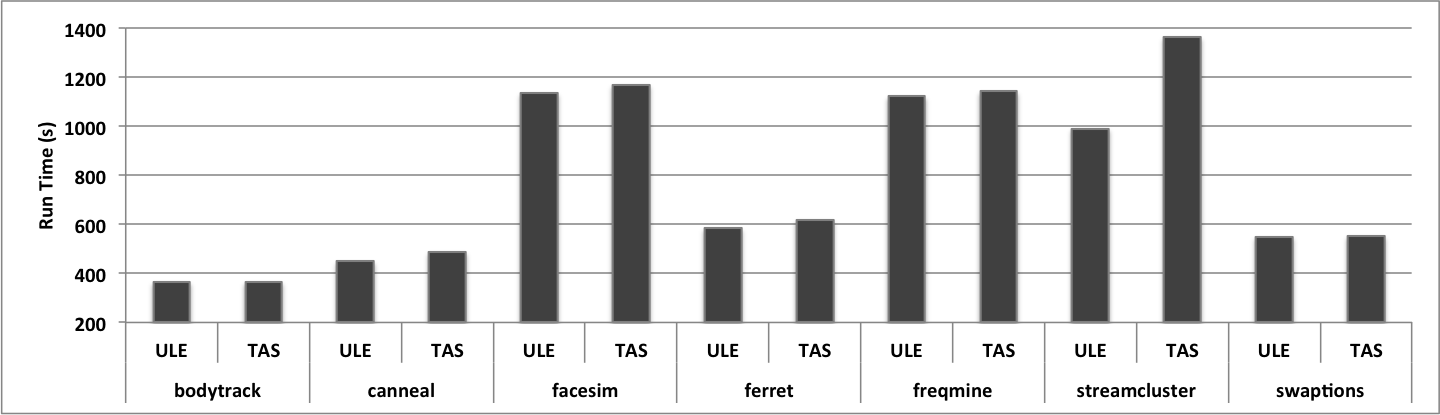
\includegraphics[width=1.0\linewidth,height=2.5in]{parsecperformance}
  \caption{Comparison of PARSEC benchmark performance under ULE and TAS
schedulers.}
  \label{fig:pbenchmarkp}
\end{figure} 
\begin{figure}[tbp]
  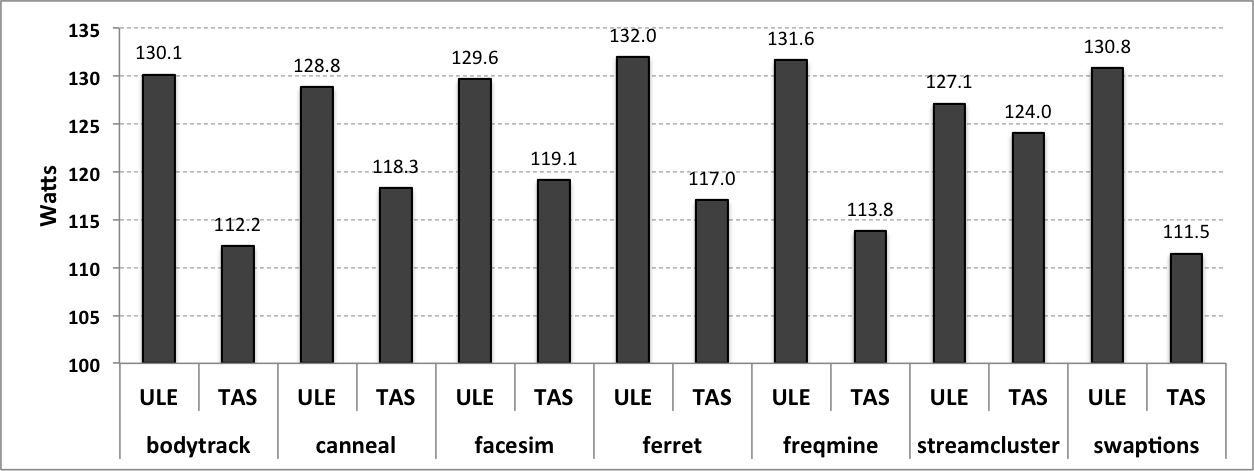
\includegraphics[width=1.0\linewidth,height=2.5in]{ParsecPowerConsumption}
  \caption{Comparison of PARSEC benchmark average power dissipation under ULE and TAS schedulers.}
  \label{fig:pbenchmark}
\end{figure}
\begin{figure}[tbp]
  \centering
  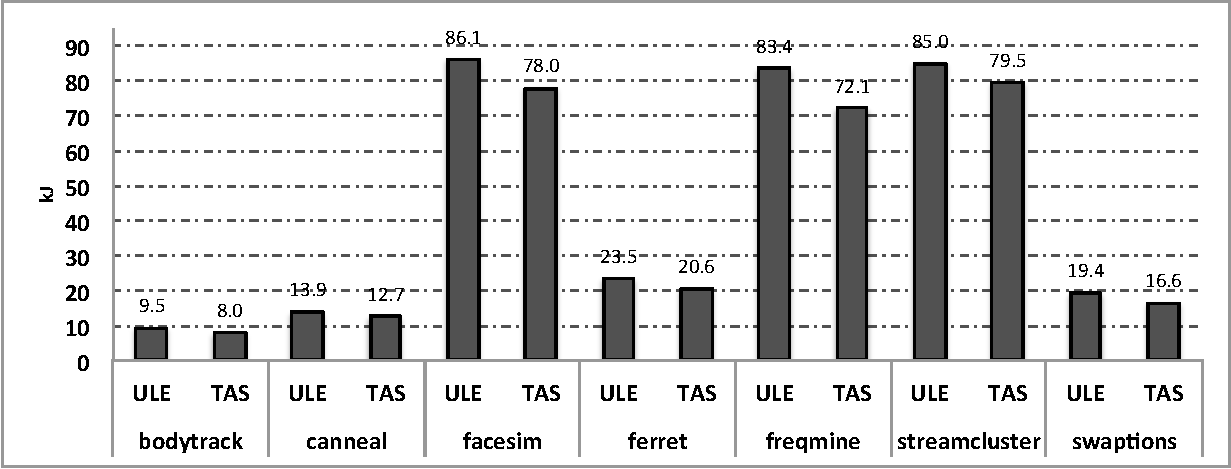
\includegraphics[width=1.0\linewidth,height=2.5in]{parseckj}
  \caption{Comparison of PARSEC total energy consumption under ULE and TAS schedulers.}
  \label{fig:penergy}
\end{figure}
Mean system power dissipation for each of the PARSEC benchmarks run on
our testbed under both schedulers is shown in
\figurename~\ref{fig:pbenchmark}.  When compared with ULE, TAS is
observed to reduce power dissipation markedly, from 14W (for the
\texttt{ferret} benchmark) to 19W (for \texttt{swaptions}), due to their
relatively small working sets.  On the other hand, less reduction in
power dissipation is found for benchmarks with large working sets,
lowering power by the range of 3W (for \texttt{streamcluster} to 10W
(for \texttt{facesim}).  The total energy consumption for each of the
PARSEC benchmarks run on our testbed is shown in
\figurename~\ref{fig:penergy}.  In comparison with ULE, TAS is observed
to reduce energy consumption between 2.8kJ (for \texttt{ferret}) to
2.9kJ (for \texttt{swaptions}) for benchmarks with relatively small
working sets, resulting in 14\% to 17\% reduction.

% In \figurename~\ref{fig:tasvsedp}, we contrast the optimization strategy
% used by TAS versus other possible optimizations schemes for managing the
% trade-off between performance and energy.  In this figure, we compare
% the energy savings from TAS for \texttt{facesim} benchmark to schemes
% that minimize delay under peak power constraints (DPC) and minimize
% energy under peak power and delay constraints (EPDC). DPC minimizes the
% delay of an execution interval so that the maximum power within an
% execution interval never exceeds a limit while EPDC schemes seek to
% minimize energy while operating a system within a power budget with a
% limit on the workload performance impact.  For the TAS results, we have
% integrated the mean power dissaption over time to compute energy use to
% compute percentage energy savings and compare against results reported
% in prior work~\cite{Cochran2011}. In this case, the optimizations used
% by TAS outperforms both DPC and EPDC for the \texttt{facesim} benchmark
% by 4\% to 6\% (against reported results in prior work of mean system
% power dissipation of 108W to 115W on a quad-core Intel processor).

% \begin{figure}[bpt]
%   \centering
% 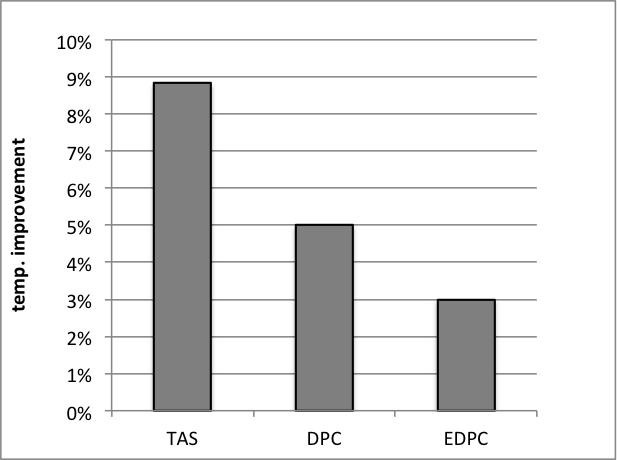
\includegraphics[width=1.0\linewidth,height=1.3in]{graphics/tasvsedpc}
%   \caption{Average percentage reduction in core die temperature for the
%     \texttt{facesim} benchmark under various optimization strategies.}
%   \label{fig:tasvsedp}
% \end{figure}
% \begin{comment}
%   Last sentence should be revised and extended per last sentence in
%   introduction. 
% \end{comment}

% Following comment block used by GNU-EMACS and AUCTEX packages
% Please do not remove.
%%% Local Variables: 
%%% mode: latex
%%% TeX-master: "dissertation.tex"
%%% TeX-PDF-mode: t
%%% TeX-source-correlate-mode: t
%%% End: 
